\begin{figure}
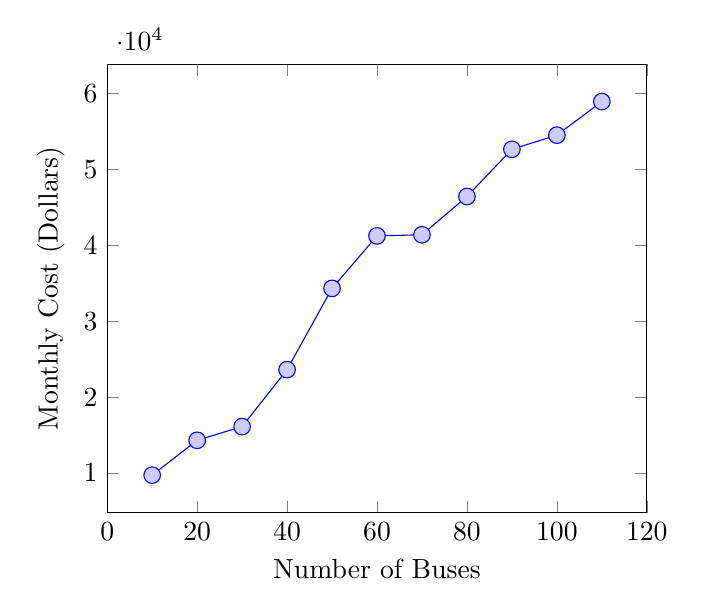
\begin{tikzpicture}
\begin{axis}[xlabel=Number of Buses, ylabel=Monthly Cost (Dollars), legend pos=north west]
	\addplot[blue] coordinates {
		(10, 9724.43)   
	  (20, 14312.58)  
		(30, 16113.51)  
		(40, 23617.81)
		(50, 34317.80)  
		(60, 41226.07)  
		(70, 41374.21) 
		(80, 46412.54)  
		(90, 52628.26)
		(100, 54490.15) 
		(110, 58912.91)}; 
\addplot[blue!20, draw=blue, only marks, mark size=3pt] coordinates {
		(10, 9724.43)   
	  (20, 14312.58)  
		(30, 16113.51)  
		(40, 23617.81)
		(50, 34317.80)  
		(60, 41226.07)  
		(70, 41374.21)  
		(80, 46412.54)  
		(90, 52628.26)
		(100, 54490.15) 
		(110, 58912.91)}; 
\end{axis}
\end{tikzpicture}
\caption{Cost comparison for different numbers of buses}
\label{fig:results:scalabilityCosts}
\end{figure}
